\documentclass[12pt]{article}

\usepackage{sbc-template}
\usepackage{graphicx,url}
\usepackage[utf8]{inputenc}
\usepackage[brazil]{babel}
\usepackage[latin1]{inputenc}  
\usepackage{xcolor}

\sloppy

\title{Vercode: Ambiente Virtual de Aprendizagem Autônomo de Programação com Recursos de Gamificação}

\author{Pedro Henrique de Jesus Silva\inst{1}, Luis Paulo da Silva Carvalho\inst{1}}

\address{Instituto Federal da Bahia (IFBA)\\
  Av. Sérgio Vieira de Melo, 3150 - Zabelê\\  
  Vitória da Conquista, Bahia, Brasil\\ 
  \email{pedrohsj.contato@gmail.com, luiscarvalho@ifba.edu.br}
}

\begin{document} 

\maketitle

\begin{abstract}
Gamification is an approach that has been increasingly used in virtual educational environments to make learning more enjoyable, engaging, and effective. This approach involves the use of game elements and mechanics in educational software, such as rewards, challenges, rankings, and badges, to encourage students to engage more with the content and achieve better results. This project aims to explore the application of gamification in the development of Vercode, a virtual education software designed for learning programming.
\end{abstract}
     
\begin{resumo} 
A gamificação é uma abordagem que tem sido cada vez mais utilizada em ambientes educacionais virtuais para tornar o aprendizado mais divertido, engajador e eficaz. Essa abordagem envolve o uso de elementos e mecânicas de jogos em softwares educacionais, tais como, recompensas, desafios, \textit{rankings} e \textit{badges}, para incentivar os alunos a se envolverem mais com o conteúdo e a alcançarem melhores resultados. Este projeto tem como objetivo explorar a aplicação da gamificação no desenvolvimento do Vercode, um software de educação virtual planejado para o aprendizado de programação.
\end{resumo}

\section{Introdução}

Compreende-se que, quando se trata de aprendizado, deve-se levar em consideração os processos que levam o conhecimento à realidade dos indivíduos e que esses processos precisam ser ajustados a essa realidade. Diante das transformações tecnológicas na sociedade, é essencial direcionar o foco do aprendizado para acompanhar os avanços. O aprendizado precisa ser estimulado através de meios multi-transdisciplinares, com o objetivo de elevar os níveis motivacionais e de engajamento \cite{TuncelAyva2010}.

Uma das práticas que vem estimulando a motivação e experiência dos usuários é a utilização e exploração de narrativas diferentes e criativas (\textit{storytelling}). De forma equivalente, os jogos são identificados como mídias capazes de motivar os indivíduos e se mostram como alternativa eficiente nesse processo de geração de conhecimento, de acordo com \cite{zichermann2011gamification} e \cite{li2012gamicad}. Jogos são capazes de promover contextos lúcidos e fictícios na forma de narrativas que favorecem a geração e relação entre conhecimentos. Agentes presentes em jogos, tais como, personagem, competição e regras podem ter efeito direto na motivação da aprendizagem, como dizem \cite{schmitz2012effects}. Portanto, pode-se perceber o poder dos jogos, quando inseridos na vida de pessoas, e que suas características apresentam resultados interessantes no que diz respeito ao processo de aprendizado e ensino.  

Gamificação pode ser definida como “a aplicação de conceitos dos jogos à vida real, com objetivo de influenciar comportamentos, melhorar a motivação e engajamento das pessoas"  \cite{marczewski2013gamification}. Como abordagem, a gamificação pode se apresentar para resolução de problemas, aumento da motivação e engajamento de determinados públicos. Sob outro ponto de vista, a gamificação pode ser entendida como um processo de melhoria de serviços, objetos ou ambientes se baseando em experiências de elementos de jogos e comportamentos dos sujeitos \cite{hamari2014does}. A educação é uma área que carece de motivação e engajamento e, portanto, a gamificação pode ter uma aplicação em contextos de ensino.

A gamificação na educação tem recebido muita atenção nos últimos anos, tanto de pesquisadores quanto de educadores. Contudo, devido à sua recente aplicação na área de educação, o conhecimento acerca do efeito da gamificação, juntamente com sua performance e o engajamento dos estudantes ainda continua escasso \cite{dicheva2015gamification}. Também de acordo com \cite{dicheva2015gamification}, alguns estudos apontam como importante a integração da gamificação em plataformas de ensino online, conhecidas como Sistemas de Gerenciamento de Aprendizagem (Learning Management Systems), ou, como é chamado no Brasil, Ambiente Virtual de Aprendizagem (AVA), nas quais são regularmente usadas como suporte no processo de aprendizado e ensino.

Tudo considerado, este trabalho teve, como objetivo, desenvolver uma plataforma online, o Vercode, que deve apresentar características e recursos da gamificação. O Vercode foi desenvolvido com o propósito de ensinar programação por meio de exercícios práticos utilizando, neste primeiro momento, a linguagem C. A plataforma apresenta uma proposta no campo da educação e do aprendizado de programação, integrando a gamificação para abordar os desafios de motivação e engajamento enfrentados por estudantes de computação ou por qualquer pessoa interessada nesta área. 

O objetivo do Vercode é criar um ambiente de aprendizado envolvente, baseado em gamificação, onde os usuários podem interagir com elementos de jogos para adquirir habilidades de programação. Ao final deste trabalho, se encontra disponibilizado como contribuição: (i) um levantamento sobre o estado da arte dos princípios e práticas da gamificação e (ii) uma prova de conceito, o Vercode, que demonstra como tais princípios podem ser concretamente implementados.

\section{Plataformas Correlatas} \label{sec:correlatos}

Alguns trabalhos similares ao Vercode ou que usam gamificação visando engajar usuários se encontram descritos nos próximos parágrafos.

A 42 School\footnote{https://www.42sp.org.br/} é uma instituição que se destaca por seu modelo de ensino baseado em projetos práticos e colaborativos, em que os alunos aprendem programação através de desafios e experiências imersivas. Eles usam alguns recursos de gamificação em sua plataforma (exemplo: conquistas e progresso).    

A DevMedia\footnote{https://www.devmedia.com.br/} é conhecida por fornecer conteúdo educacional em programação através de tutoriais e cursos online também aplicando os conceitos de gamificação.

O Duolingo\footnote{https://pt.duolingo.com/} é amplamente reconhecido por sua abordagem inovadora no ensino de idiomas, usando gamificação para tornar o aprendizado de línguas mais eficaz e agradável.

Em comparação com as plataformas correlatas, esta pesquisa proporciona como vantagens: (i) um estudo sobre os princípios de gamificação e aplicação dos princípios, (ii) código-fonte disponibilizado para evoluir, estudar e melhorar o Vercode e (iii) fornecer uma plataforma específica para a comunidade de desenvolvedores, com desafios e projetos práticos que são diretamente relevantes para a carreira em TI. Isso torna a programação acessível a um público mais amplo e diversificado, promovendo a inclusão e a igualdade de oportunidades. 

\section{O Vercode} \label{sec:vercode}

O Vercode é uma plataforma online, desenvolvida pelo autor principal deste trabalho, que atua sobre o ensino e aprendizado de programação e que utiliza recursos da gamificação. Neste trabalho, o Vercode é utilizado como uma prova de conceito para aplicação dos princípios de gamificação  (mais detalhes na Seção 4).

A ideia se originou de uma escola de programação chamada 42 (mencionada nos trabalhos correlatos, Seção 2). A 42, originalmente da França, criou um conceito de escola diferente, onde não existem professores e nem aulas, os alunos percorrem uma trilha de conteúdos e exercícios e vai aprendendo em conjunto com outros estudantes, este também utiliza de alguns recursos de gamificação. 

O foco da 42 é explorar a capacidade de aprender e evoluir em conjunto, já o Vercode tem mais ênfase na gamificação e seus benefícios. Seu propósito é fornecer um ambiente virtual lúdico e criativo, para aumentar o engajamento e interesse de cada usuário.

O público alvo são pessoas que estejam interessadas em aprender a programar, ou quem já teve um contato com programação, mas apresentou dificuldade no aprendizado. No entanto, é importante notar que qualquer usuário familiarizado com os conceitos dos jogos virtuais pode encontrar uma imersão natural na plataforma. O que se pretende é que a gamificação traga uma flexibilidade ao Vercode, permitindo que ele atenda a um amplo espectro de públicos.

\subsection{Princípios de Gamificação} \label{sec:principios}

Gamificação é um conceito utilizado para resolução de problemas através da ascendência e aperfeiçoamento do engajamento por meio de estímulos à motivação particular do indivíduo \cite{busarello2016gamification}. 

O principal papel da gamificação é se apropriar de elementos dos jogos para aplicar os mesmos em outros contextos, em produtos e serviços, que não necessariamente são focados em jogos, mas tem a intenção de proporcionar motivação e estimular o comportamento de usuários. A gamificação na educação tem recebido muita atenção nos últimos anos, tanto de pesquisadores quanto educadores. Contudo, devido à sua recente aplicação na área de educação, o conhecimento acerca do efeito da gamificação, juntamente com o engajamento dos estudantes ainda continua escasso \cite{dicheva2015gamification}. 

O cérebro humano pode se beneficiar das experiências oferecidas pelos jogos, tais como resolver enigmas e receber resposta, pois são estímulos que ativam o sistema de dopamina no cérebro, associado à atividade ao prazer, de acordo \cite{clementi2014diretrizes}. Além disso, em um jogo o indivíduo tem a oportunidade de vencer desafios e perder, mas não de forma permanente. O jogador sempre terá a oportunidade de refazer a tarefa, buscando seu êxito. Isso serve como motivador para uma busca constante de melhorias e maneiras novas para se encontrar soluções \cite{busarello2016gamification}

A gamificação é formada por princípios que tem base nos jogos, nas suas mecânicas e estética. Entretanto, o foco é o engajamento das pessoas, na promoção do aprendizado e na solução de problemas. De acordo com \cite{ludospro}, alguns desses princípios são:

\begin{enumerate}
    \item \textit{\textbf{Storytelling}}: a arte de contar histórias. É uma prática que busca desenvolver histórias ou narrativas, que tem como objetivo educar e entreter. No cenário da gamificação, esse elemento é usado para engajar o público-alvo e criar um interesse no conteúdo que está sendo compartilhado;
    \item \textit{\textbf{Ranking}}: um sistema de ranking serve para identificar os melhores colocados na atividade, destacando aqueles que mais compreenderam o conteúdo apresentado. Ele serve para sustentar a competição e estimular interesse por parte dos participantes em se esforçar para alcançar melhores colocações;
    \item \textbf{Desafios}: o que motiva os participantes a se esforçarem para alcançar a meta da atividade são os desafios, mas, para que isto funcione, três recursos precisam ser trabalhados: desafio, conquistas e missões, que geram interesse nos participantes para que se mantenham voluntária e ativamente na atividade. Ademais, é preciso equilibrar o nível de dificuldade da prática sugerida para que o participante entenda que consegue atingir o que foi apresentado. O contrário também precisa ser considerado. É importante que o usuário não veja o desafio como fácil demais, porque isso vai gerar desânimo e, consequentemente, falta de engajamento;
    \item \textbf{Recompensa}: outra abordagem muito presente nos jogos é a recompensa, que ocorre de acordo com cada reação positiva/correta do jogador. Este também é um recurso para estimular o interesse do participante, por isso precisa ser implementado de maneira totalmente estratégica para cumprir com o seu papel. Pode-se utilizar diferentes formas de recompensa: (i) avançar para uma próxima etapa, (ii) moedas, (iii) pontos e (iv) medalhas virtuais que possam ser trocadas por outros itens, (v) barra de experiência que cresce conforme cada conquista concluída, entre outros;
    \item \textbf{Pontos}: pontos são considerados um sistema de recompensa que denotam aos participantes seu progresso no processo e aumenta sua motivação com as práticas. A cada acerto uma certa quantidade de pontos vai ser contabilizada e, conforme a dificuldade for aumentando, maior também poderá ser a recompensa. Dessa forma, o jogador tem uma motivação para se desafiar cada vez mais e com isso cumprir a meta final da estratégia de gamificação. Esse mecanismo também é usado para gerar um sentimento de competição entre os participantes, principalmente quando trabalhado junto ao \textit{ranking};
    \item \textbf{Mecânicas}: são um conjunto ou bloco de regras cruciais utilizadas no processo da gamificação. As mecânicas sozinhas não são suficientes para transformar uma experiência dada em uma engajada, mas são auxiliadoras para que isso aconteça;
    \item \textbf{Estética}: a estética condiz com o olhar e o sentir da experiência, que são fundamentais para o processo da gamificação. Interpreta a maneira como a experiência é esteticamente assimilada pelo indivíduo. Bons recursos visuais, áudio e animação podem tornar um jogo mais agradável e manter os jogadores ainda mais envolvidos.
\end{enumerate}

O fundamento nos jogos se dá na criação de um sistema ou ambiente em que os indivíduos queiram investir seu tempo e energia. Assim como nos jogos, o pensamento é o atributo mais importante da gamificação. Isso corresponde à ideia de converter uma tarefa tediosa e desinteressante em uma atividade incentivadora, aplicando elementos gamificados, tais como, cooperação, exploração, competição e narrativa. O pensamento se transforma em um gerenciador de fatos virtuais que promovem percepções em operações no mundo real \cite{kapp2012gamification}. 

\subsection{Prototipagem} \label{sec:prototipagem}

O desenvolvimento do Vercode foi iniciado pela prototipação da interface de usuário. A prototipagem antes da criação do software é uma etapa importante para garantir o sucesso do projeto. Segundo Pressman (2015), a prototipagem ou MVP (Mínimo Produto Viável), permite aos desenvolvedores e às partes interessadas obterem uma compreensão mais clara dos requisitos do software. Através da criação de um protótipo, é possível visualizar e interagir com as funcionalidades e o fluxo do software antes do desenvolvimento completo. Isso ajuda a identificar problemas ou discrepâncias nos requisitos iniciais, permitindo que sejam ajustados antes de investir tempo e recursos significativos.
	
A prototipagem também contribui para a economia de tempo e recursos, conforme destacado por \cite{somerville2003engenharia}. Ao criar um protótipo, é possível identificar e resolver problemas de usabilidade, funcionalidade ou design de forma mais rápida e eficiente do que na fase de desenvolvimento completo. Isso reduz o retrabalho e os custos associados ao desenvolvimento de um software que não atende aos requisitos ou às expectativas dos usuários. O restante desta seção discute os resultados obtidos através da prototipagem.

A Figura \ref{fig:tela_usuario} exibe a tela do usuário. Nela encontram-se componentes e cada um deles tem características e princípios diferentes de gamificação, que serão descritos e analisados nos próximos parágrafos. Ou seja, os itens gamificados da Figura \ref{fig:tela_usuario} serão  particionados e detalhados pelas descrições das figuras seguintes.  

\begin{figure}[ht!]
\centering
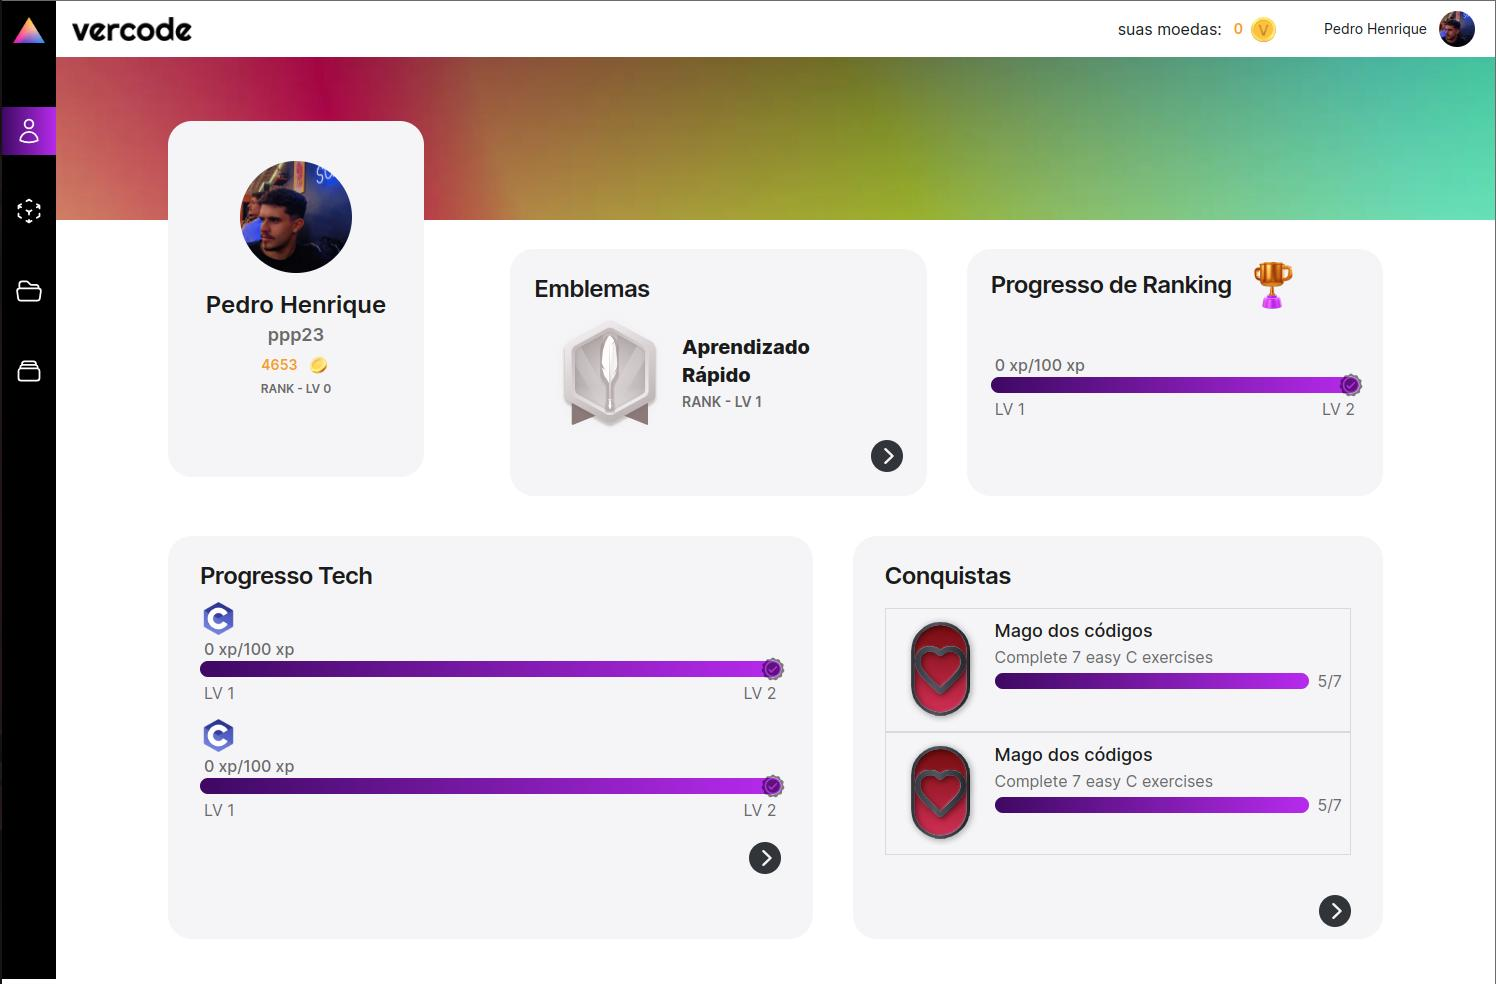
\includegraphics[width=1.0\textwidth]{imagens/tela_usuario.jpg}
\caption{Tela de usuário da plataforma Vercode}
\label{fig:tela_usuario}
\end{figure}

A Figura \ref{fig:cartao_usuario} mostra um cartão do usuário, que mostra algumas informações: nome (“Pedro Henrique”), nome de usuário (“ppp23”), quantidade de moedas (“4653”) e o progresso atual (“RANK - LV 0”). Neste exemplo, a informação sobre o progresso e moedas aponta para o princípio de \textbf{pontos} que foi abordado na Seção 4. 

\begin{figure}[ht!]
\centering
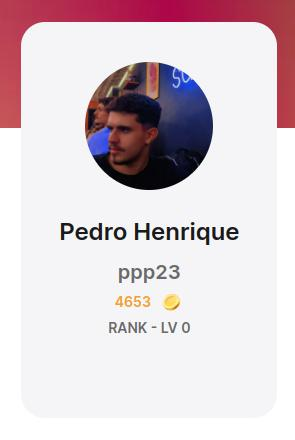
\includegraphics[width=0.42\textwidth]{imagens/cartao_usuario.jpg}
\caption{Cartão do Usuário}
\label{fig:cartao_usuario}
\end{figure}

Figura \ref{fig:cartao_emblemas} é visualizado o cartão de emblemas que apresenta o nome (“Aprendizado Rápido”), a informação do progresso atual (“RANK - LV1”), a imagem do emblema atual daquele usuário, e, por fim, um botão para ver todos os emblemas com detalhes. Na figura, portanto, pode-se encontrar o princípio da \textbf{recompensa} sendo operacionalizado através dos emblemas.

\begin{figure}[ht!]
\centering
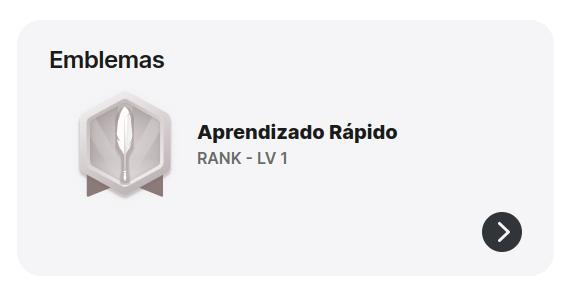
\includegraphics[width=0.5\textwidth]{imagens/cartao_emblemas.jpg}
\caption{Emblemas do Usuário}
\label{fig:cartao_emblemas}
\end{figure}

A Figura \ref{fig:cartao_progresso} contém  um recorte gráfico do componente de progresso. Nele é possível visualizar a quantidade de pontos de experiência que um usuário tem e quantos pontos são necessários para subir para o próximo nível (“0 xp/100 xp”). Tem-se uma barra de progresso visual que mostra também esse valor. Neste exemplo, por estar com 0 pontos de experiência a barra roxa não aparece. Com isso, mais uma vez, pode ser visto o princípio de \textbf{pontos} sendo implementado. 

\begin{figure}[ht!]
\centering
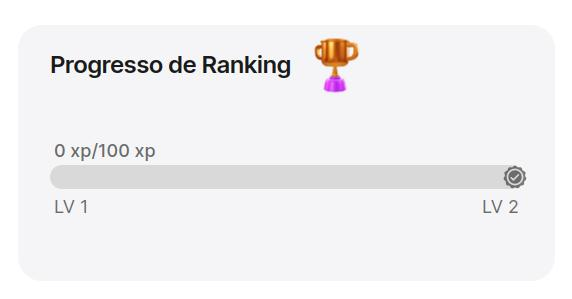
\includegraphics[width=0.5\textwidth]{imagens/progresso.jpg}
\caption{Progresso do Usuário}
\label{fig:cartao_progresso}
\end{figure}

O protótipo do Vercode foi discutido com o orientador e também autor deste trabalho durante encontros sucessivos até que foi atingido um consenso sobre sobre sua estética (outro princípio apontado na Seção 4) e funcionalidades gamificadas. Posterior a isto, iniciou-se o desenvolvimento, que se encontra descrito nas próximas seções.

\subsection{Arquitetura do Vercode} \label{sec:arquitetura}

A aplicação foi dividida entre front-end e back-end, não sendo, portanto, um projeto monolítico. 

A Figura \ref{fig:arquitetura} ilustra a arquitetura do Vercode. Nela, tem-se a conexão do usuário, representado na figura como “Cliente”, através de um navegador web com a interface da plataforma, o front-end. Para se conectar com o back-end, o front-end utiliza o protocolo HTTP para troca de informações.

O back-end é composto pela lógica de negócio, o motor de gamificação e a conexão com o banco de dados. A camada de dados gerencia os registros de cada usuário e demais informações necessárias para uso pelo motor de gamificação. Além de oferecer exercícios práticos, o Vercode também realiza a correção dos códigos escritos pelos usuários. Essa correção inclui a execução e compilação de códigos, os quais podem variar de linguagem ao longo do tempo. O Vercode suporta uma ampla gama das principais linguagens de programação utilizadas no mercado, abrangendo aquelas suportadas pelo Judge0. O Judge0\footnote{https://judge0.com/} é um serviço open source, que executa os código e devolve uma resposta para o back-end a fim de avaliar o resultado e fornecer um feedback para o usuário, seja ele negativo ou positivo, o recompensando. O Judge0 foi desenvolvido com o propósito de ser um sistema de execução de código on-line robusto, escalável e de código aberto que pode ser usado para construir uma ampla variedade de aplicativos que precisam de recursos de execução de código.

Existe também a conexão de "STORE FILES" com o serviço da AWS. Nesse serviço são armazenados todos os arquivos necessários para serem mostrados ao usuário no front-end. Por exemplo, as imagens utilizadas para os emblemas ("\textit{badges}").   
   
\begin{figure}[ht!]
\centering
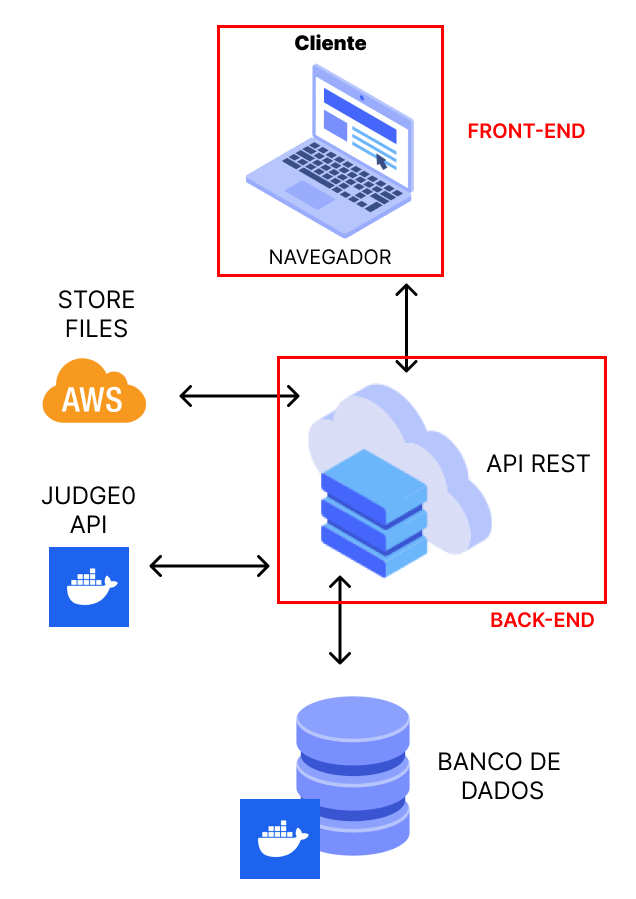
\includegraphics[width=.6\textwidth]{imagens/arquitetura_vercode.png}
\caption{Arquitetura do Vercode}
\label{fig:arquitetura}
\end{figure}

\subsection{O Front-end} \label{sec:front_end}

O front-end é a camada na qual acontece a programação de toda parte visual e interativa que o usuário terá com o Vercode. Tecnologias como React\footnote{https://react.dev/} e Next.js\footnote{https://nextjs.org/} foram utilizadas para construção dos componentes visuais. A linguagem de programação utilizada foi o Typescript\footnote{https://www.typescriptlang.org/}, linguagem atual baseada em Javascript e que traz a possibilidade de programação orientada a objetos. A parte da estilização, e consequente implementação do princípio de \textbf{estética}, ficou por conta do Tailwind\footnote{https://tailwindcss.com/} que é um framework CSS para escrever estilos dentro do HTML.

Nessa fase, o enfoque foi direcionado à criação dos componentes e páginas da plataforma. Por exemplo, foram desenvolvidas páginas de aprendizado, módulos de gamificação e perfis de usuário, que são essenciais para um fluxo de usabilidade. Foram utilizados dados mockados\footnote{Dados falsos, estáticos, utilizados somente para prototipagem e testes rápidos} durante o desenvolvimento enquanto ainda não existia um back-end (mais detalhes na Seção 5.3), simulando informações fictícias que representam o comportamento esperado dos dados reais. Isso permitiu testar e iterar rapidamente sobre a experiência do usuário. O uso de dados mockados possibilitou simular o comportamento do back-end enquanto o front-end estava sendo desenvolvido.

Importante ressaltar que a fase de criação do front-end somente se iniciou após o protótipo visual ter atingido um consenso (Seção 5.1).

\subsection{O Back-end} \label{sec:back_end}

O back-end do Vercode, foi projetado utilizando uma API REST, que permite receber requisições HTTP vindas do cliente, processar essas informações e devolver uma resposta para esses pedidos. As ferramentas utilizadas foram o Nest.js\footnote{https://nestjs.com/}, um framework baseado em Node.js\footnote{https://nodejs.org/en} para construção de back-ends eficientes, confiáveis e escaláveis do lado do servidor. Por ser baseado em Node.js foi mantida a escolha do Typescript como linguagem também no back-end. O PostgreSQL\footnote{https://www.postgresql.org/} foi utilizado como banco de dados, por ser  open source e disponibilizado sem custos.

Como é possível ver na Figura \ref{fig:tabelas}, o modelo do banco de dados centraliza-se em torno do usuário (tabela destacada em vermelho). A partir dele tem-se diversas relações “muitos-para muitos” e tabelas importantes para dar suporte à gamificação (na cor verde): emblemas (“badges), progresso\_tecnologias (“tech\_progress”), exercícios(“exercises”), projeto (“project”), nível (“level”), progresso\_rank (“rank\_progress”) e eventos (“events”). Para cada uma dessas tabelas é prevista outra intermediária (todas destacadas em amarelo) para relacionar os dados da gamificação com os usuários.  Por exemplo, saber o status em que cada usuário está durante a realização de seus exercícios/desafios.

\begin{figure}[ht!]
\centering
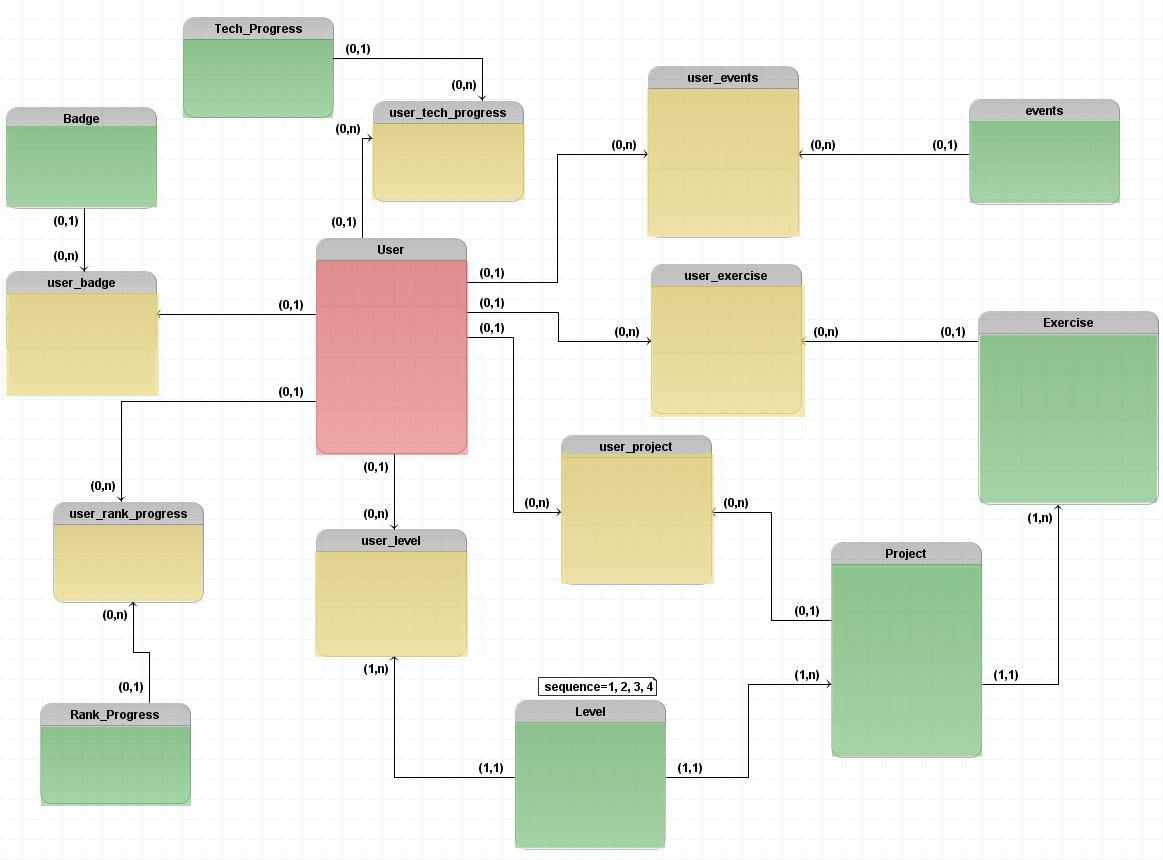
\includegraphics[width=1.0\textwidth]{imagens/tabelas.jpg}
\caption{Esquema lógico do banco de dados do Vercode}
\label{fig:tabelas}
\end{figure}

A etapa final envolveu a integração do front-end com o back-end. Foram configuradas conexões com a API do Nest.js para acessar dados do PostgreSQL, substituindo gradualmente os dados mockados por informações reais. Nesta etapa, também garantiu-se que as rotas da API no back-end estivessem configuradas adequadamente para atender às solicitações do front-end. Tal abordagem de desenvolvimento permitiu que o Vercode evoluísse de um protótipo funcional com dados fictícios (ou mockados) para uma plataforma completa e interconectada. O back-end também contou com a integração com a ferramenta de compilação de código, o Judge0. 

\subsection{O Resultado Final} \label{sec:resultado_final}

As telas apresentadas a seguir mostram o resultado final do funcionamento do Vercode juntamente com os conceitos de gamificação que foram aplicados. 

A Figura \ref{fig:projetos} exibe a tela de projetos do Vercode. Nela é possível visualizar todos os projetos disponíveis para aquele usuário. Os projetos representam, no contexto do Vercode, a implementação do princípio de gamificação, \textbf{desafios}.

\begin{figure}[ht!]
\centering
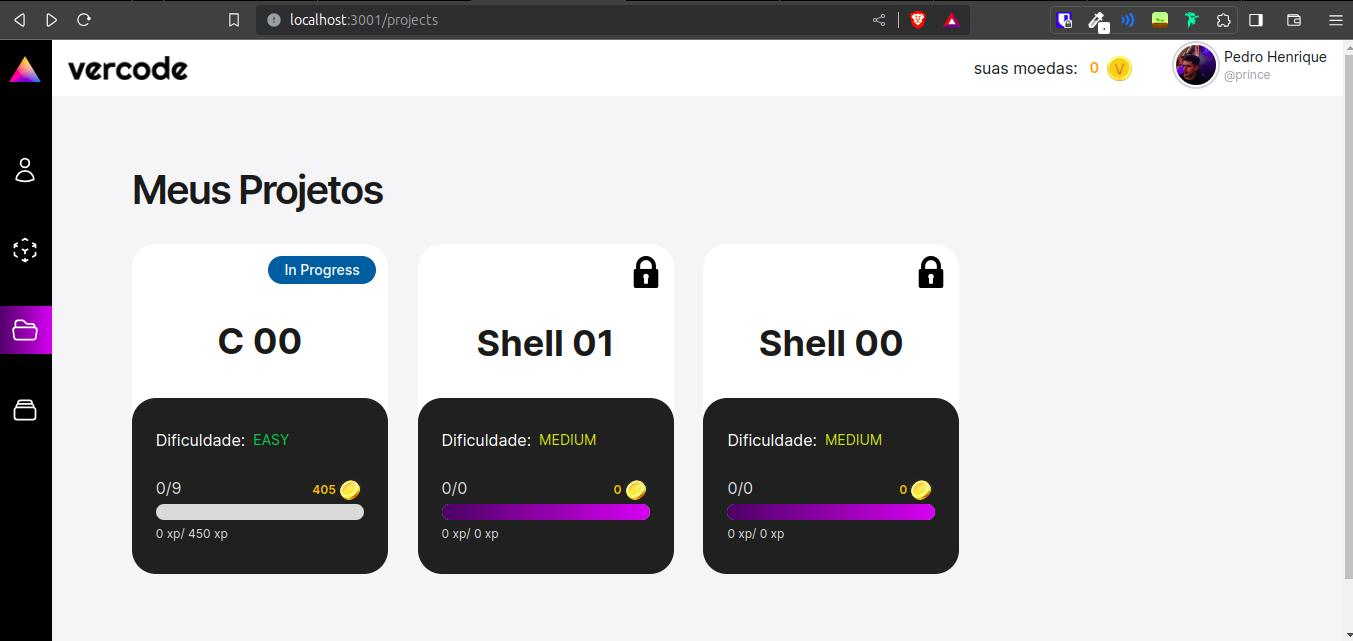
\includegraphics[width=1.0\textwidth]{imagens/tela_projetos.jpg}
\caption{Tela de Projetos do Vercode}
\label{fig:projetos}
\end{figure}

A Figura \ref{fig:cartao_projeto} exibe mais detalhes sobre um projeto/desafio. A figura exibe o título do projeto, “C 00”, o seu status atual, indicado pela tag azul “in progress” (“Em progresso”), o nível de dificuldade, “easy” ("fácil), e uma barra de progresso com alguns detalhes, tais como quantidade de exercícios contidos naquele projeto, “0/9”, a quantidade total de moedas que será ganha quando finalizar o projeto, “405”, e, por fim, a quantidade de pontos de experiência atual em relação ao total, “0 xp/450 xp”. Aqui temos o exemplo de alguns elementos de gamificação: \textbf{recompensas} e \textbf{pontos}.

\begin{figure}[ht!]
\centering
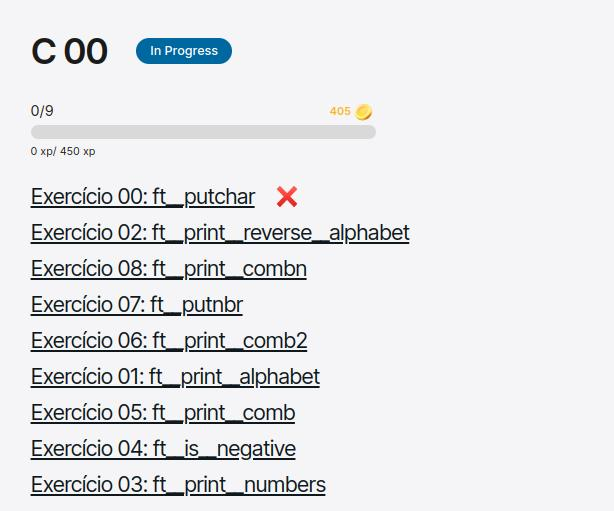
\includegraphics[width=0.5\textwidth]{imagens/cartao_projeto.jpg}
\caption{Cartão de um Projeto}
\label{fig:cartao_projeto}
\end{figure}

Na Figura \ref{fig:tela_codificacao} é possível observar a tela de codificação do projeto proposto como desafio. A Figura mostra as informações básicas de cada exercício, tais como, nome, “Exercício 00: ft\_putchar”, e recompensas por aquele exercício: quantidade de moedas e pontos de experiência e os pontos de experiência relativos à linguagem de programação que está sendo usada no exercício atual. É possível ver também as instruções para guiar o usuário a resolver o problema apresentado, e por fim um editor de código para que o usuário possa digitar a sua resposta.

\begin{figure}[ht!]
\centering
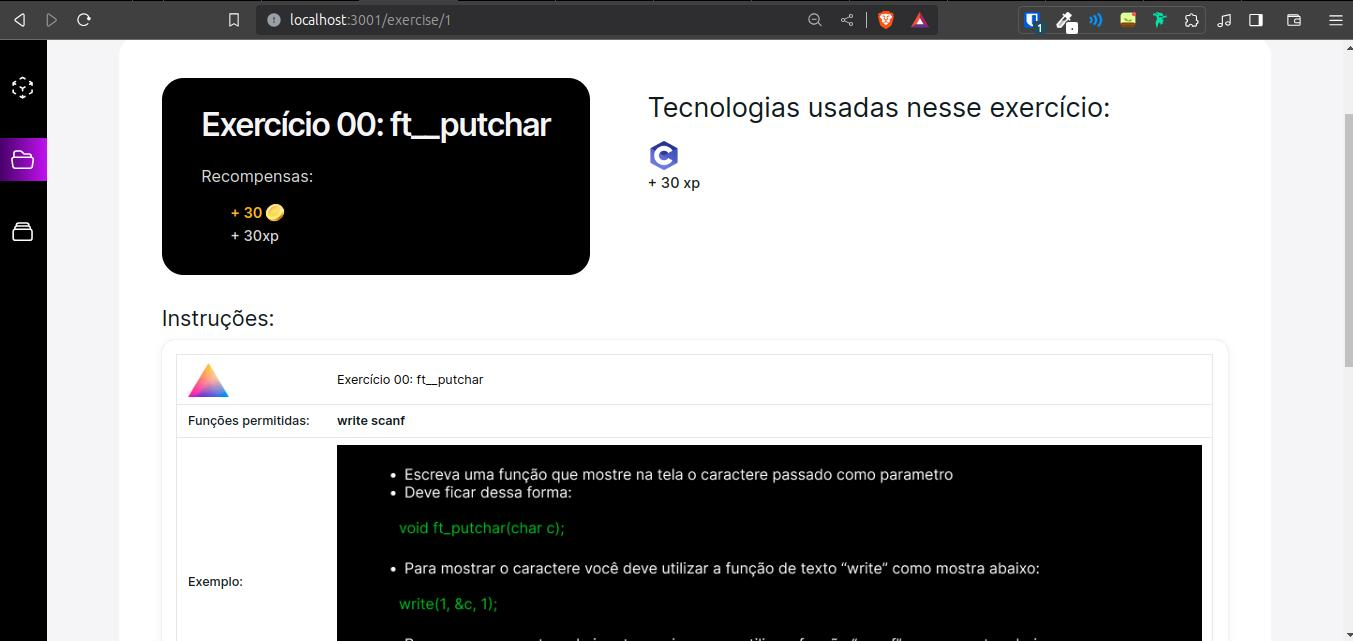
\includegraphics[width=1.0\textwidth]{imagens/resolucao_desafio.jpg}
\caption{Tela de Codificação}
\label{fig:tela_codificacao}
\end{figure}

Na Figura \ref{fig:feedback_incorreta}, tem-se um feedback quando a resolução do problema de codificação não ocorre de forma correta. A mensagem é apresentada de forma não agressiva, encorajando o usuário a tentar novamente. Isto corresponde à implementação de outro princípio de gamificação, o \textbf{engajamento}, com a intenção de não desmotivar, indicando a possibilidade de novas tentativas. 

\begin{figure}[ht!]
\centering
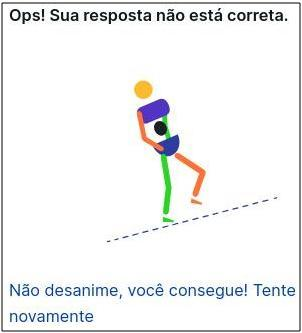
\includegraphics[width=0.5\textwidth]{imagens/feedback_resposta_incorreta.jpg}
\caption{Resultado do exercício em caso de resposta errada}
\label{fig:feedback_incorreta}
\end{figure}

A Figura \ref{fig:feedback_correta} mostra um feedback positivo da resolução do problema de codificação. A mensagem comemora o sucesso (princípio de \textbf{engajamento}) e busca evidenciar o que o usuário ganhou com a resolução do problema (princípios de \textbf{pontos} e \textbf{emblemas}). 

\begin{figure}[ht!]
\centering
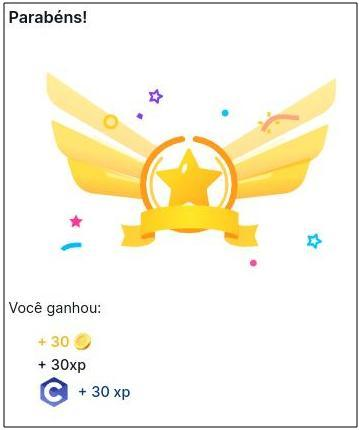
\includegraphics[width=0.5\textwidth]{imagens/feedback_resposta_correta.jpg}
\caption{Resultado do exercício em caso de resposta correta}
\label{fig:feedback_correta}
\end{figure}

Em todo o processo de submissão de código de projetos, com o gerenciamento da compilação, validação, feedbacks e pontuações/emblemas, tem-se o conceito de \textbf{mecânicas} aplicado. 

Com a aplicação finalizada, ela foi hospedada em nuvem, visando a realização de testes pelos autores deste trabalho. O serviço de compilação de código, Judge0 está hospedados em serviços da AWS\footnote{https://aws.amazon.com/pt/} (\textit{Amazon Web Services}). Além disso, para armazenar imagens e demais arquivos, também foi utilizada a AWS, mais especificamente o serviço Bucket S3.

\section{Considerações Finais} \label{sec:consideracoes_finais}

Ao longo deste trabalho, foi feito o estudo da aplicação da gamificação em uma plataforma de aprendizado de programação. Buscou-se utilizar a gamificação para criar um ambiente de aprendizado envolvente. A gamificação foi implementada para estimular o interesse, incentivar a participação ativa e criar uma comunidade colaborativa na plataforma.

Como prova de conceito, foi desenvolvido  o Vercode, uma plataforma de aprendizado de programação, enfatizando a gamificação como catalisador para o engajamento dos usuários. As bases teóricas e as tendências observadas na literatura sugerem que a gamificação tem o potencial de aumentar o engajamento dos nossos usuários e promover uma experiência educacional mais positiva. Através da integração de elementos de jogos, a abordagem apresentada buscou criar um ambiente com potencial para estimular  o interesse dos usuários no aprendizado de programação.

Embora o conteúdo deste trabalho tenha sido aplicado, na forma de prova de conceito, ao Vercode somente, o que foi apresentado pode ser replicado para criar outros softwares gamificados. Isso se dá pelo fato de ter sido utilizado um padrão de arquitetura de software genérico e bem difundido atualmente, front-end e back-end, e a demonstração da integração deste tipo de arquitetura com os princípios de gamificação. Qualquer trabalho futuro que use este como referência poderá aproveitar o exemplo do Vercode e especificá-lo para aplicar gamificação em algum outro nicho específico.

\subsection{Trabalhos Futuros} \label{sec:futuro}

Há várias direções promissoras para expandir e aprimorar o Vercode no futuro. 

Não foi possível durante a idealização e construção do Vercode, realizar testes de satisfação com usuários que tiveram acesso à plataforma, podendo assim verificar a eficácia da gamificação e se existe o engajamento por parte do uso. Uma validação com usuário finais não foi realizada pois não tinha sido definida e conceituada no escopo inicial do projeto. Apenas os autores deste trabalho testaram e evoluíram o Vercode com os testes. 

Outras frentes de trabalho  se encontram a seguir:

\begin{enumerate}
    \item \textbf{Melhoria Contínua da Experiência do Usuário}: investir em design de interface do usuário e usabilidade para tornar a plataforma ainda mais intuitiva e amigável sob o contexto dos princípios de gamificação elencados na Seção 4. Por exemplo, como melhor representar a evolução dos pontos alcançados a cada desafio? Como engajar mais os usuários para que eles ganhem mais pontos usando o Vercode? 
    \item \textbf{Análise de Dados Avançada}: implementar técnicas de análise de dados avançadas para entender melhor os padrões de aprendizado dos usuários, identificar áreas de melhoria e personalizar a experiência do usuário através da gamificação;
    \item \textbf{Acessibilidade}: garantir acessibilidade para usuários com necessidades especiais, promovendo um ambiente verdadeiramente inclusivo. Personalizar os  princípios de gamificação e,  consequentemente, engajar usuários com necessidades especiais;
    \item \textbf{Estabelecimento de Conexões Online}: criação de um sistema robusto de conexões online e interações gamificadas entre estudantes. Isso poderia ser realizado através da implementação de fóruns de discussão temáticos, salas de chat, ou colaboração em projetos de programação. Isto iria requerer, possivelmente, evoluir a pesquisa sobre gamificação para entender como seus princípios podem englobar colaboração entre usuários;
    \item \textbf{Adição de \textit{Ranking}}: Introduzir um sistema de \textit{ranking} comparativo entre usuários. Ao permitir que os estudantes se comparam com seus pares em termos de pontuações, conquistas e progresso, talvez seja possível criar uma atmosfera de competição. Todavia, deve ser investigado como os princípios de gamificação podem ser adaptados para permitir que isto ocorra de forma saudável;
    \item \textbf{Correção de Exercícios}: Introduzir um sistema mais completo e complexo na análise de algoritmos enviados pelos usuários. Atualmente o código de resolução feito pelos estudantes é compilado e seu resultado é analisado. Entretanto, para uma experiência mais completa e que evite tentativas de “burlar” o mecanismo de correção. Isto é importante para  que o mecanismo de pontuação seja justo para cada um dos usuários  de um software gamificado.
\end{enumerate}

\subsection{Contribuições} \label{sec:contribuicoes}

Durante condução do trabalho e ao finalizá-lo, algumas contribuições foram realizadas. A primeira delas, o código-fonte do Vercode no Github\footnote{https://github.com/vercodeorg/vercode}, se encontra acessível pelo QR-Code contido na Figura \ref{fig:qrcode_codigo}.
    
\begin{figure}[ht!]
\centering

\includegraphics[width=0.5\textwidth]{imagens/qrcode_codigo.png}
\caption{Código fonte do Vercode no Github}
\label{fig:qrcode_codigo}
\end{figure}

Foi realizada na disciplina de IHM (Interface Homem Máquina) uma apresentação sobre este trabalho, a fim de exemplificar e mostrar os conceitos da gamificação e sua aplicação. A palestra teve como objetivo demonstrar a realização prática de temas e assuntos realacionados à disciplina, por exemplo, usabilidade e interatividade, já que a gamificação motiva o usuário e gera engajamento.

\newpage

\bibliographystyle{sbc}
\bibliography{bibliografia}

\newpage

\noindent\textbf{Apêndice}

Os conceitos adquiridos durante o curso de Bacharelado em Sistemas de Informação (BSI) pelo Instituto Federal de Educação, Ciência e Tecnologia da Bahia contribuíram para a construção do projeto, desde o levantamento teórico até a aplicação prática. 

A Figura \ref{fig:disciplinas} demonstra todas as disciplinas que contemplam a ementa do curso de BSI e que se relacionam de forma direta e indireta na minha visão.

\begin{figure}[ht!]
\centering
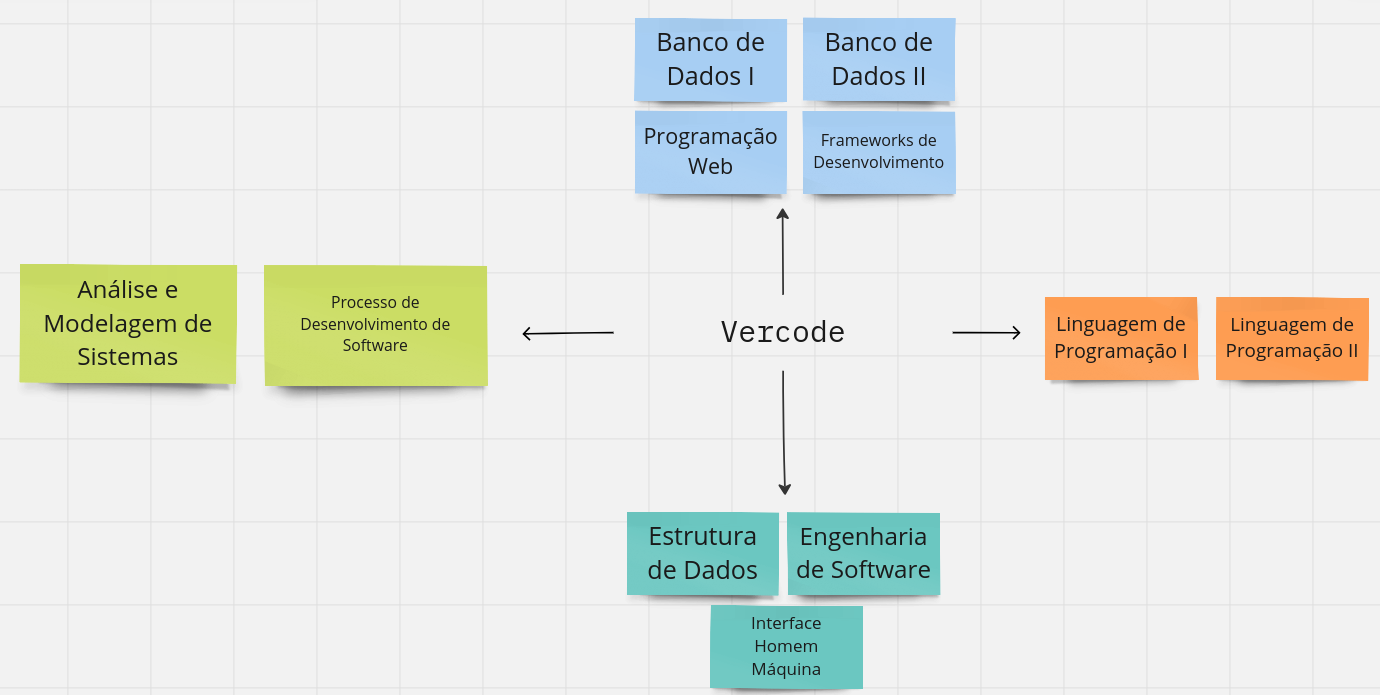
\includegraphics[width=1.0\textwidth]{imagens/disciplinas.png}
\caption{Disciplinas do curso de BSI relacionadas a aplicação do projeto}
\label{fig:disciplinas}
\end{figure}

\end{document}
